\chapter{Dipole Antenna}
In the previous chapter we discussed the Hertz dipole which is a small current element and we concluded that it is not an effective radiator because the radiation resistance is very small. However, the Hertz dipole creates a foundation to discuss practical complex antenna structures. In this chapter we would investigate the radiation characteristics (radiation patterns) of a linear thin dipole. 

\section{Analysis of the thin wire dipole}
Essentially, the thin wire dipole is a piece of wire with length comparable to the wavelength of the time varying current. The basic arrangement is shown in figure\ref{figure1} below. In a simplistic way, it is possible to think of the antenna as having formed by bending the two wires of an open-ended transmission line down and up by $90^\circ$. The mid point, at which the bends occur, is known as the feed point. 
\begin{figure}[h]
\centering
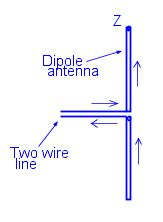
\includegraphics[height=5cm]{./graphics/diagram5}
\caption{A thin dipole antenna driven sinusoidally by a two wire line}
\label{figure1}
\end{figure}

If we consider a transmission line which is open circuited at one end, we can visualize the standing wave patterns on this transmission line as shown in \ref{figure2}a. Now, Flaring up the ends to $90^\circ$ such that it is a dipole, we can still visualize the standing wave patterns of current on the structure as shown, which is maintained. 
\begin{figure}[h]
\centering
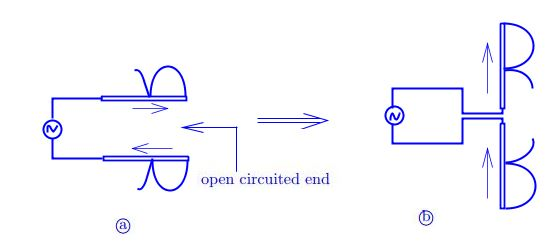
\includegraphics[width=1\linewidth]{./graphics/diagram6}
\caption{a. Open circuited TL with current standing wave pattern shown.           
 b. Flared up version of the TL with current standing wave pattern shown for an ideal case dipole}
\label{figure2}
\end{figure}

We might argue that for a completely flared up transmission line, are the standing wave patterns valid? Yes, they are, because the rigorous solution for the current distribution on the dipole is the same kind as that we get from the standing wave pattern on a transmission line. A few things to note are:
\begin{enumerate}[(i)]
\item  At the top of the antenna the current must go to zero because there is no path for the current at the tip of the antenna.
\item  There is symmetry of current in the transmission line as equal current flow in opposite direction through the two and in essence there is symmetry of the current distribution in the dipole. 
\end{enumerate}

It is important to note that the input terminal current is decided by the length of the antenna and is independent of the voltage excitation. The reason is if the current goes to zero at the top of tip of the antenna then for different lengths of the antenna, the input current would not be the same irrespective of the given voltage source.

In conclusion, for a thin wire dipole, the current distribution though not proven here, has symmetry on the dipole, reduces to zero at the tip of the antenna and is a function of the length of the dipole.

Let us consider a dipole antenna aligned in the z direction as shown in \ref{figure3} below, which has a current I(z) that is flowing through it. 
\begin{figure}[h]
\centering
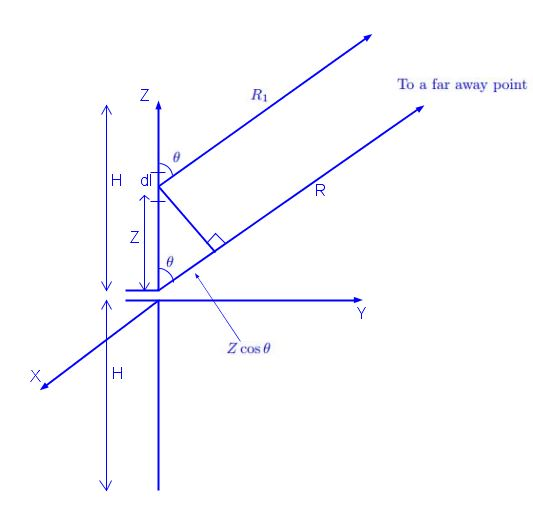
\includegraphics[height=5cm]{./graphics/diagram7}
\caption{A dipole antenna aligned in the z - direction}
\label{figure3}
\end{figure}

We will visualize the dipole antenna as the collection of the Hertz dipoles and consider a Hertz dipole I(z)dz at a distance z from the feed point. Let us determine the fields at a far away point due to the small current element (because we are concerned with radiation fields) that makes an angle of $\theta$ with the z axis. Since we are considering a far away point, the two lines in \ref{figure3} appear parallel and the difference in distance traveled by waves along this path is given by $zcos\theta$. This means the radiation from the Hertz dipole with respect to the centre leads in phase by $zcos\theta$ because it travels lesser distance than that from the centre. We get from \ref{figure3} that $R - z\cos\theta = R_1. \ R_1$ is the distance from the observation point from the origin. 

The current distribution for the dipole antenna fed at the centre is given by
$$I(z) = I_m\sin \{\beta(H -|z|)\} = \begin{cases} I_m\sin{\beta(H - z)}& \text{$z > 0,$}\\
I_m\sin{\beta(H + z)}&\text{$z < 0$}	\end{cases}
$$
With the current distribution we will find the fields at a far away point, a distance $R_1$ from the source - a small current element $I(z)dz$. We recall that the fields $(E\&H)$ produced at a point from the source is given by 
$$
\fbox{$
dE_\theta = j\dfrac{\beta^2\sin\theta}{4\pi\omega\epsilon} \times \dfrac{I(z)dz}{R_1}e^{-j\beta R_1} $} \ \ 
\footnote{neglecting the time varying element $e^{j\omega t}$}
$$
And we know that the wave generated is essentially a transverse electromagnetic wave so, magnetic field $dH_\phi = \dfrac{dE_\theta}{\eta}$

Let us calculate the electric field
$$
dE_\theta = j\dfrac{\beta^2\sin\theta}{4\pi\omega\epsilon} \times \dfrac{I(z)}{R - z\cos\theta}e^{-j\beta(R - z\cos\theta)}\ dz
$$
For far away points, the denominator $R - z\cos\theta \approx\ R$ since $R \gg H$ (condition for far fields)
$$ So, \quad
dE_\theta = j\dfrac{\beta^2\sin\theta}{4\pi\omega\epsilon} \times \dfrac{I(z)}{R}e^{-j\beta(R - z\cos\theta)}\ dz
$$ 
To find the total field, we superpose the field contributed by each small current element which is the integral from -H to +H.
$$
E_\theta = \int^{+H}_{-H}\left[j\dfrac{\beta^2\sin\theta}{4\pi\omega\epsilon} \times
\dfrac{I(z)}{R}e^{-j\beta(R - z\cos\theta)}\ dz \right]
$$
$$
= j\dfrac{\beta^2\sin\theta}{4\pi R\omega\epsilon}\int^{+H}_{-H}
I(z)e^{-j\beta(R - z\cos\theta)}\ dz
$$
$$
= j\dfrac{\beta^2\sin\theta}{4\pi R\omega\epsilon}e^{-j\beta R}\int^{+H}_{-H}
I(z)e^{j\beta z\cos\theta}\ dz
$$
$$
E_\theta= j\dfrac{\beta^2\sin\theta}{4\pi R\omega\epsilon}e^{-j\beta R}\int^{+H}_{-H}
I_m\sin[\beta(H - |z|)]e^{j\beta z\cos\theta}\ dz
$$
$$
= \left[\dfrac{j\beta^2I_me^{-j\beta R}\sin\theta}{4\pi R\omega\epsilon}\right]\int^{+H}_{-H}
\sin[\beta(H - |z|)]e^{j\beta z\cos\theta}\ dz
$$
Let us denote the constants from the integral by K that is, $K = \dfrac{j\beta^2I_me^{-j\beta R}\sin\theta}{4\pi R\omega\epsilon}$ 
$$
E_\theta = K\int^{+H}_{-H}
\sin[\beta(H - |z|)]e^{j\beta z\cos\theta}\ dz\\
$$
From Euler's identity, $e^{j\beta z\cos\theta} = \cos(\beta z\cos\theta) + j\sin(\beta z\cos\theta)$
\begin{dmath*}
So, \ \ E_\theta = K\int^{+H}_{-H}
\sin[\beta(H - |z|)]\left[\cos(\beta z\cos\theta) + j\sin(\beta z\cos\theta)\right]\ dz
\end{dmath*}
\begin{dmath*}
= K\int^{+H}_{-H}\left[\
\sin[\beta(H - |z|)]\cos(\beta z\cos\theta)dz + j\sin[\beta(H - |z|)]\sin(\beta z\cos\theta)dz \ \right]
\end{dmath*}
To simplify the solution, we identify the odd and even functions in the expression because the integral from -H to +H of an odd function reduces to zero by using the conditions, $f(-x) = f(x)\longrightarrow even; f(-x) = -f(x)\longrightarrow odd$ \\\\
$\sin[\beta(H - |z|)] \longrightarrow even\ function,\ because, f(-z) = f(z)\\\\
\cos(\beta z\cos\theta)\longrightarrow even\ function,\ because, f(-z) = f(z)\\\\ and  \ 
 \sin(\beta z\cos\theta)\longrightarrow odd\ function,\ because, f(-z) = -f(z)
$

In the integral, the imaginary term reduces to zero as it is an odd function ($odd \times even = odd$). So the expression simplifies to 
$$
E_\theta = K\int^{+H}_{-H}\sin[\beta(H - |z|)]\cos(\beta z\cos\theta)\ dz
$$
$$
recall \ that \sin \{\beta(H - \mid z\mid)\} = \begin{cases} I_m\sin{\beta(H - z)}& \text{$z > 0,$}\\
I_m\sin{\beta(H + z)}&\text{$z < 0$}	\end{cases}
$$
\begin{dmath*}
E_\theta = K\left[ \int^0_{-H}\sin[\beta(H + z)]\cos(\beta z\cos\theta)\ dz + 
\int^H_0\sin[\beta(H - z)]\cos(\beta z\cos\theta)\ dz \right]
\end{dmath*}

Due to symmetry,$$ E_\theta = 2K\int^H_0\sin[\beta(H - z)]\cos(\beta z\cos\theta)\ dz $$
Using trigonometric identities,
$$
\sin A\cos B = \dfrac{1}{2}\{\sin(A + B) + \sin(A - B)\}
$$
\begin{dmath*}
E_{\theta} =2K\int_{0}^{H} \dfrac{1}{2}\left\lbrace\sin(\beta(H-z) +\beta z\cos \theta) + \sin(\beta(H-z) - \beta z\cos \theta) \right\rbrace dz
\end{dmath*}
\begin{dmath*}
=K\ \int_{0}^{H}\left\lbrace\sin(\beta[H-z+z\cos \theta]) + \sin(\beta[H-z-z\cos \theta])\right \rbrace dz
\end{dmath*}
\begin{dmath*}
=K\int_{0}^{H}\left\lbrace\sin(\beta z(\cos \theta -1) + \beta H)+ {\sin(\beta z(1 + \cos \theta) - \beta H)}\right\rbrace dz
\end{dmath*}
\begin{dmath*}
=K\left\lbrace \left.-\dfrac{1}{\beta(\cos\theta -1)} \cos(\beta z(\cos\theta -1) + \beta H) \right|_{0}^{H} +\left. \dfrac{1}{\beta(\cos \theta + 1)} \cos(\beta z(\cos\theta + 1) - \beta H)\right|_{0}^{H} \right\rbrace
\end{dmath*}
\begin{dmath*}
\hspace{-50pt}=K\left\lbrace-\dfrac{1}{\beta(\cos\theta -1)} \cos(\beta H(\cos\theta -1) + \beta H) + \dfrac{1}{\beta(\cos\theta -1)} \cos(\beta H) - \dfrac{1}{\beta(\cos\theta + 1)} \cos(\beta H) +\dfrac{1}{\beta(\cos\theta + 1)} \cos(\beta H(\cos\theta + 1) -\beta H)\right\rbrace
\end{dmath*}
\begin{dmath*}
=K\left\lbrace -\dfrac{1}{\beta(\cos \theta -1)} \cos(\beta H \cos\theta) + \dfrac{1}{\beta(\cos\theta - 1)} \cos(\beta H) - \dfrac{1}{\beta(\cos\theta + 1)} \cos(\beta H) + \dfrac{1}{\beta(\cos\theta + 1)} \cos(\beta H \cos\theta)\right\rbrace
\end{dmath*}
\begin{dmath*}
=K\left\lbrace\cos(\beta H\cos \theta)\left[\dfrac{1}{\beta(\cos \theta + 1)}- \dfrac{1}{\beta(\cos\theta - 1)}\right] + \cos \beta H\left[\dfrac{1}{\beta(\cos\theta  - 1)} - \dfrac{1}{\beta(\cos\theta + 1)}\right]\right\rbrace
\end{dmath*}
$$=K\left\lbrace\dfrac{\cos(\beta H\cos \theta)}{\beta} \left[\dfrac{2}{\sin^{2}\theta}\right] + \cos \beta H\left[\dfrac{-2}{\sin^{2}\theta}\right] \right\rbrace$$
$$=2K \left\lbrace\dfrac{\cos(\beta h\cos\theta) - \cos\beta H}{\beta\sin^{2}\theta}\right\rbrace$$
Let's replace K
$$E_{\theta} = \dfrac{j\beta I_m}{2\pi W\epsilon}\left\{\dfrac{\cos(\beta H\cos \theta)- \cos \beta H}{\sin\theta}\right\} \dfrac{e^{-j\beta R}}{R}$$
\begin{align}
=E_\circ F(\theta) \dfrac{e^{-j\beta R}}{R}
\label{eqn12}
\end{align}
where $$E\circ= \dfrac{j\beta I_m}{2\pi \omega\epsilon} ,\ \beta=\omega\sqrt{\mu_o} \epsilon_o$$ 
$$ =\dfrac{jI_m\eta}{2\pi}, \eta =120\pi$$
$$E_\circ= j60I_m $$
The expression in equation \ref{eqn12} gives the variation of amplitude as a function of R and it varies inversely as R, the distance from the center of the dipole, which is the same as the case of the Hertz dipole. There is also a phase term $\textbf(e^{j\beta R})$ which represents a wave traveling in the R direction at a distance R from the source.

Since we are interested in the radiation pattern we have seen that we use the normalized expression of the fields to determine the radiation pattern so we will concern ourselves with the function $F(\theta)$ given by:
$$F(\theta) = \dfrac{\cos(\beta H\cos\theta) - \cos \beta H}{\sin \theta}$$
From the previous chapters  it was said that we would assume that the radiation pattern for the H-plane is circular and so our investigation is only for the E-plane. Also we would like to know the input impedance for a certain length of the dipole antenna from the given expression for the current distribution. If we assume an excitation voltage of 1volts then the input impedance $Z_{\textnormal{in}} = \dfrac{1}{I_{\textnormal{m}} \sin \beta H}$\footnote{because $Z_{in}=\frac{V}{I}$ where $I = I_m\sin\beta$ H at $z= 0$.}
It should be noted that the input impedance which is a measure of power radiated by the antenna is now a complex quantity and now depends on the value of H of the dipole and may vary over a very wide range as $\sin \beta H$ changes from $0 \rightarrow 1$ or $\beta H$ changes from $0\rightarrow\dfrac{\pi}{2}$. For $\beta H = \frac{\pi}{2},\ \frac{3\pi}{2},\ \ldots$ $Z_{\textnormal{in}}=\frac{1}{I_{\textnormal{m}}}$ but at $\beta H = 0, \pi\ \ldots Z_{\textnormal{in}} =\infty$, so the range of values of $Z_{\textnormal{in}}$ is ${\frac{1}{I_m}}\rightarrow \infty$ at H values of ${\frac{\lambda}{4}} \rightarrow \frac{\lambda}{2}$ $(\beta H = \frac{2 \pi H}{\lambda})$

The values of H are not unique values because $\sin \beta H$ goes to zero or 1 again for another $2\pi$ revolution i.e $\beta H \pm 2m\pi$. So there are multiples of length the antenna can take. Now that it is obvious that there is no precise value length for the variation of input impedance, what happens to the radiation pattern when the length changes? From the expression of $F(\theta)$, if the values of H varies, $F(\theta)$ might have multiple maxima and might go to zero many times. In investigating the radiation pattern we will consider those cases where there are no electric fields and conclude that in between 2 consecutive directions where the electric field has gone to zero there must be a maxima and this approach is easier as the calculation of the direction of the maximum of electric field is a rather tedious task. The direction where the electric field goes to zero is called the direction of nulls.

So, to get the direction of nulls we equate $F(\theta)$ to zero;
$$F(\theta) = \dfrac{\cos(\beta H \cos \theta) - \cos \beta H}{\sin \theta} = 0$$
implies
$$\cos(\beta H \cos \theta) = \cos(\beta H)$$
$$\beta H \cos \theta = \pm \beta H \pm 2m\pi\footnote{If the cosine of angles are equal then it is equal for multiple revolutions of the angles.}$$ where m = 0, 1, 2$\ldots$
$$\cos \theta = \pm 1 \pm \frac{2m\pi}{\beta H}\ldots$$
$$= \pm 1 \pm \frac{2m\pi}{\dfrac{2\pi H}{\lambda}}$$
\begin{align}
\cos\theta = \pm1 \pm \frac{m\lambda}{H}
\label{eqn13}
\end{align}
which gives the direction of nulls.
Firstly, for a given value of H, we consider all values of m for which $\cos \theta$ is less than or equal to 1 and that gives the direction of nulls. From the expression of equation \ref{eqn13} , it can be noticed that as H increases, there are more values of m where there will be $\cos \theta \leq 1$ which means there will be multiple direction of nulls. However, for m = 0 , $\cos \theta = \pm 1$ which corresponds to $\theta = 0$ or $\theta =\pi$. So there should be a null at these directions but from $ F(\theta)$, the denominator goes to zero, then we cannot be certain of nulls at these directions.
\paragraph{}
To know if indeed $F(\theta)$ goes to zero at $\theta = 0$ or $\theta = \pi$ we take limits (L'Hopital rule)
\begin{dmath*}
\lim\limits_{\theta \rightarrow 0}{ \dfrac{\cos(\beta H \cos \theta) - \cos \beta H}{\sin \theta}} = \left.\dfrac{-\beta H \sin \theta \cos(\beta H \cos \theta)}{\cos \theta}\right |_{\theta=0, \theta = \pi}
=0
\end{dmath*}
this shows there is indeed a null at these directions which makes sense, because the dipole is a collection of the Hertz dipole and the Hertz dipole has a null along its axis i.e  $\theta = 0$ and $\theta = \pi$, so the super-position of the field should also have a null in these directions. This also shows that the dipole is not radiating in the direction along its axis.

Now, let's take specific cases for different lengths of the antenna.\\
\textbf{Case 1}: $H =\dfrac{\lambda}{4}$, height of dipole = $2H = \dfrac{\lambda}{2}$\\
$\cos = \pm1 \pm \dfrac{m\lambda}{\dfrac{\lambda}{4}} = \pm1 \pm 4m$ which corresponds to having a null only at $m = 0$ that is at $\theta = 0$ or $\theta = \pi$. Remember we are considering cases of $\cos\leq1$ because the range of values of of $\cos \theta$ is $0\rightarrow1$. The plot of the  pattern is shown in figure \ref{figure4} which is the same as that of the Hertz dipole.
\begin{figure}[h]
\centering
\includegraphics[width=1\linewidth]{"./graphics/fig 4 lec 10"}
\caption{E - plane radiation pattern of $2H = \dfrac{\lambda}{2}$}
\label{figure4}
\end{figure}

\textbf{Case 2}:$H = \dfrac{\lambda}{2}$, height of dipole $=2H =\lambda$\\
$\cos \theta = \pm 1 \pm \dfrac{m\lambda}{\dfrac{\lambda}{2}} = \pm 1 \pm 2m$
Also $\theta = 0$ or $\pi$ which gives a radiation pattern that is the same as case 1, though it is compressed as shown below. 
\begin{figure}[h]
\centering
\includegraphics[width=1\linewidth]{"./graphics/fig 5 lecture 10"}
\caption{E - plane radiation pattern of $2H = \lambda$}
\label{figure5}
\end{figure}

\textbf{Case 3}: $H = \dfrac{3\lambda}{4}$, height of dipole $2H = \dfrac{3\lambda}{2}$\\
$$\cos \theta = \pm1 \pm \dfrac{m\lambda}{\dfrac{3\lambda}{4}} = \pm 1\pm \dfrac{4m}{3}$$
Firstly, we get the nulls for $m=0$ which is $\theta = 0$ or $\theta = \pi$. Next, we set $m=1$ and choosing the sign appropriately we get $\cos \theta = =\dfrac{4}{3} - 1$ or $+1-\dfrac{4}{3}=\pm\frac{1}{3}$. So, $\theta = \arccos(\pm \dfrac{1}{3})$
this gives the radiation pattern shown in figure\ref{figure6}.
\begin{figure}[h]
\centering
\includegraphics[width=1\linewidth]{"./graphics/fig 6 lec 48"}
\caption{E - plane radiation pattern of $2H = \dfrac{3\lambda}{2}$}
\label{figure6}
\end{figure}

Therefore it shows that as the value of H increases, there will be more nulls and the radiation pattern becomes more complicated.\\
\textbf{Case 4}: $H = \lambda$, height of dipole $ =2H = 2\lambda$\\
$\cos \pm 1 \pm \dfrac{m\lambda}{\lambda} = \pm1 \pm m$ which gives nulls for $m = 0$ and $m= 1$ at $\theta =0$ or $\theta = \pi$ and $\theta = \dfrac{\pi}{2}$ and the radiation pattern is shown in figure\ref{figure7}
\begin{figure}[h]
\centering
\includegraphics[width=1\linewidth]{"./graphics/fig 7 eplane"}
\caption{E - plane radiation pattern for $2H = 2\lambda$}
\label{figure7}
\end{figure}

In conclusion, as the length of the dipole increases the radiation pattern gets more modified with more nulls and also varies the input impedance of the dipole antenna. Now, let's move on to discuss the radiation characteristics of an antenna.